\section{Project Description}
The aim of this project is to produce the electronics for a set of headphones which will be capable of detecting and cancelling an unwanted sound source from that being heard by the user.
\\
\\
There are many distractions in the world today, and almost every single one of them produces sound of some sort.
These sounds can be disturbing from trying to hear a specific sound, such as a telephone call.
However not all of these sounds are unwanted.
Headphones exist on the market to cancel out all the sounds hitting the ear, so that only the sound being produced by them is heard, but they do not account for other sounds.
\begin{figure}
	\centering
	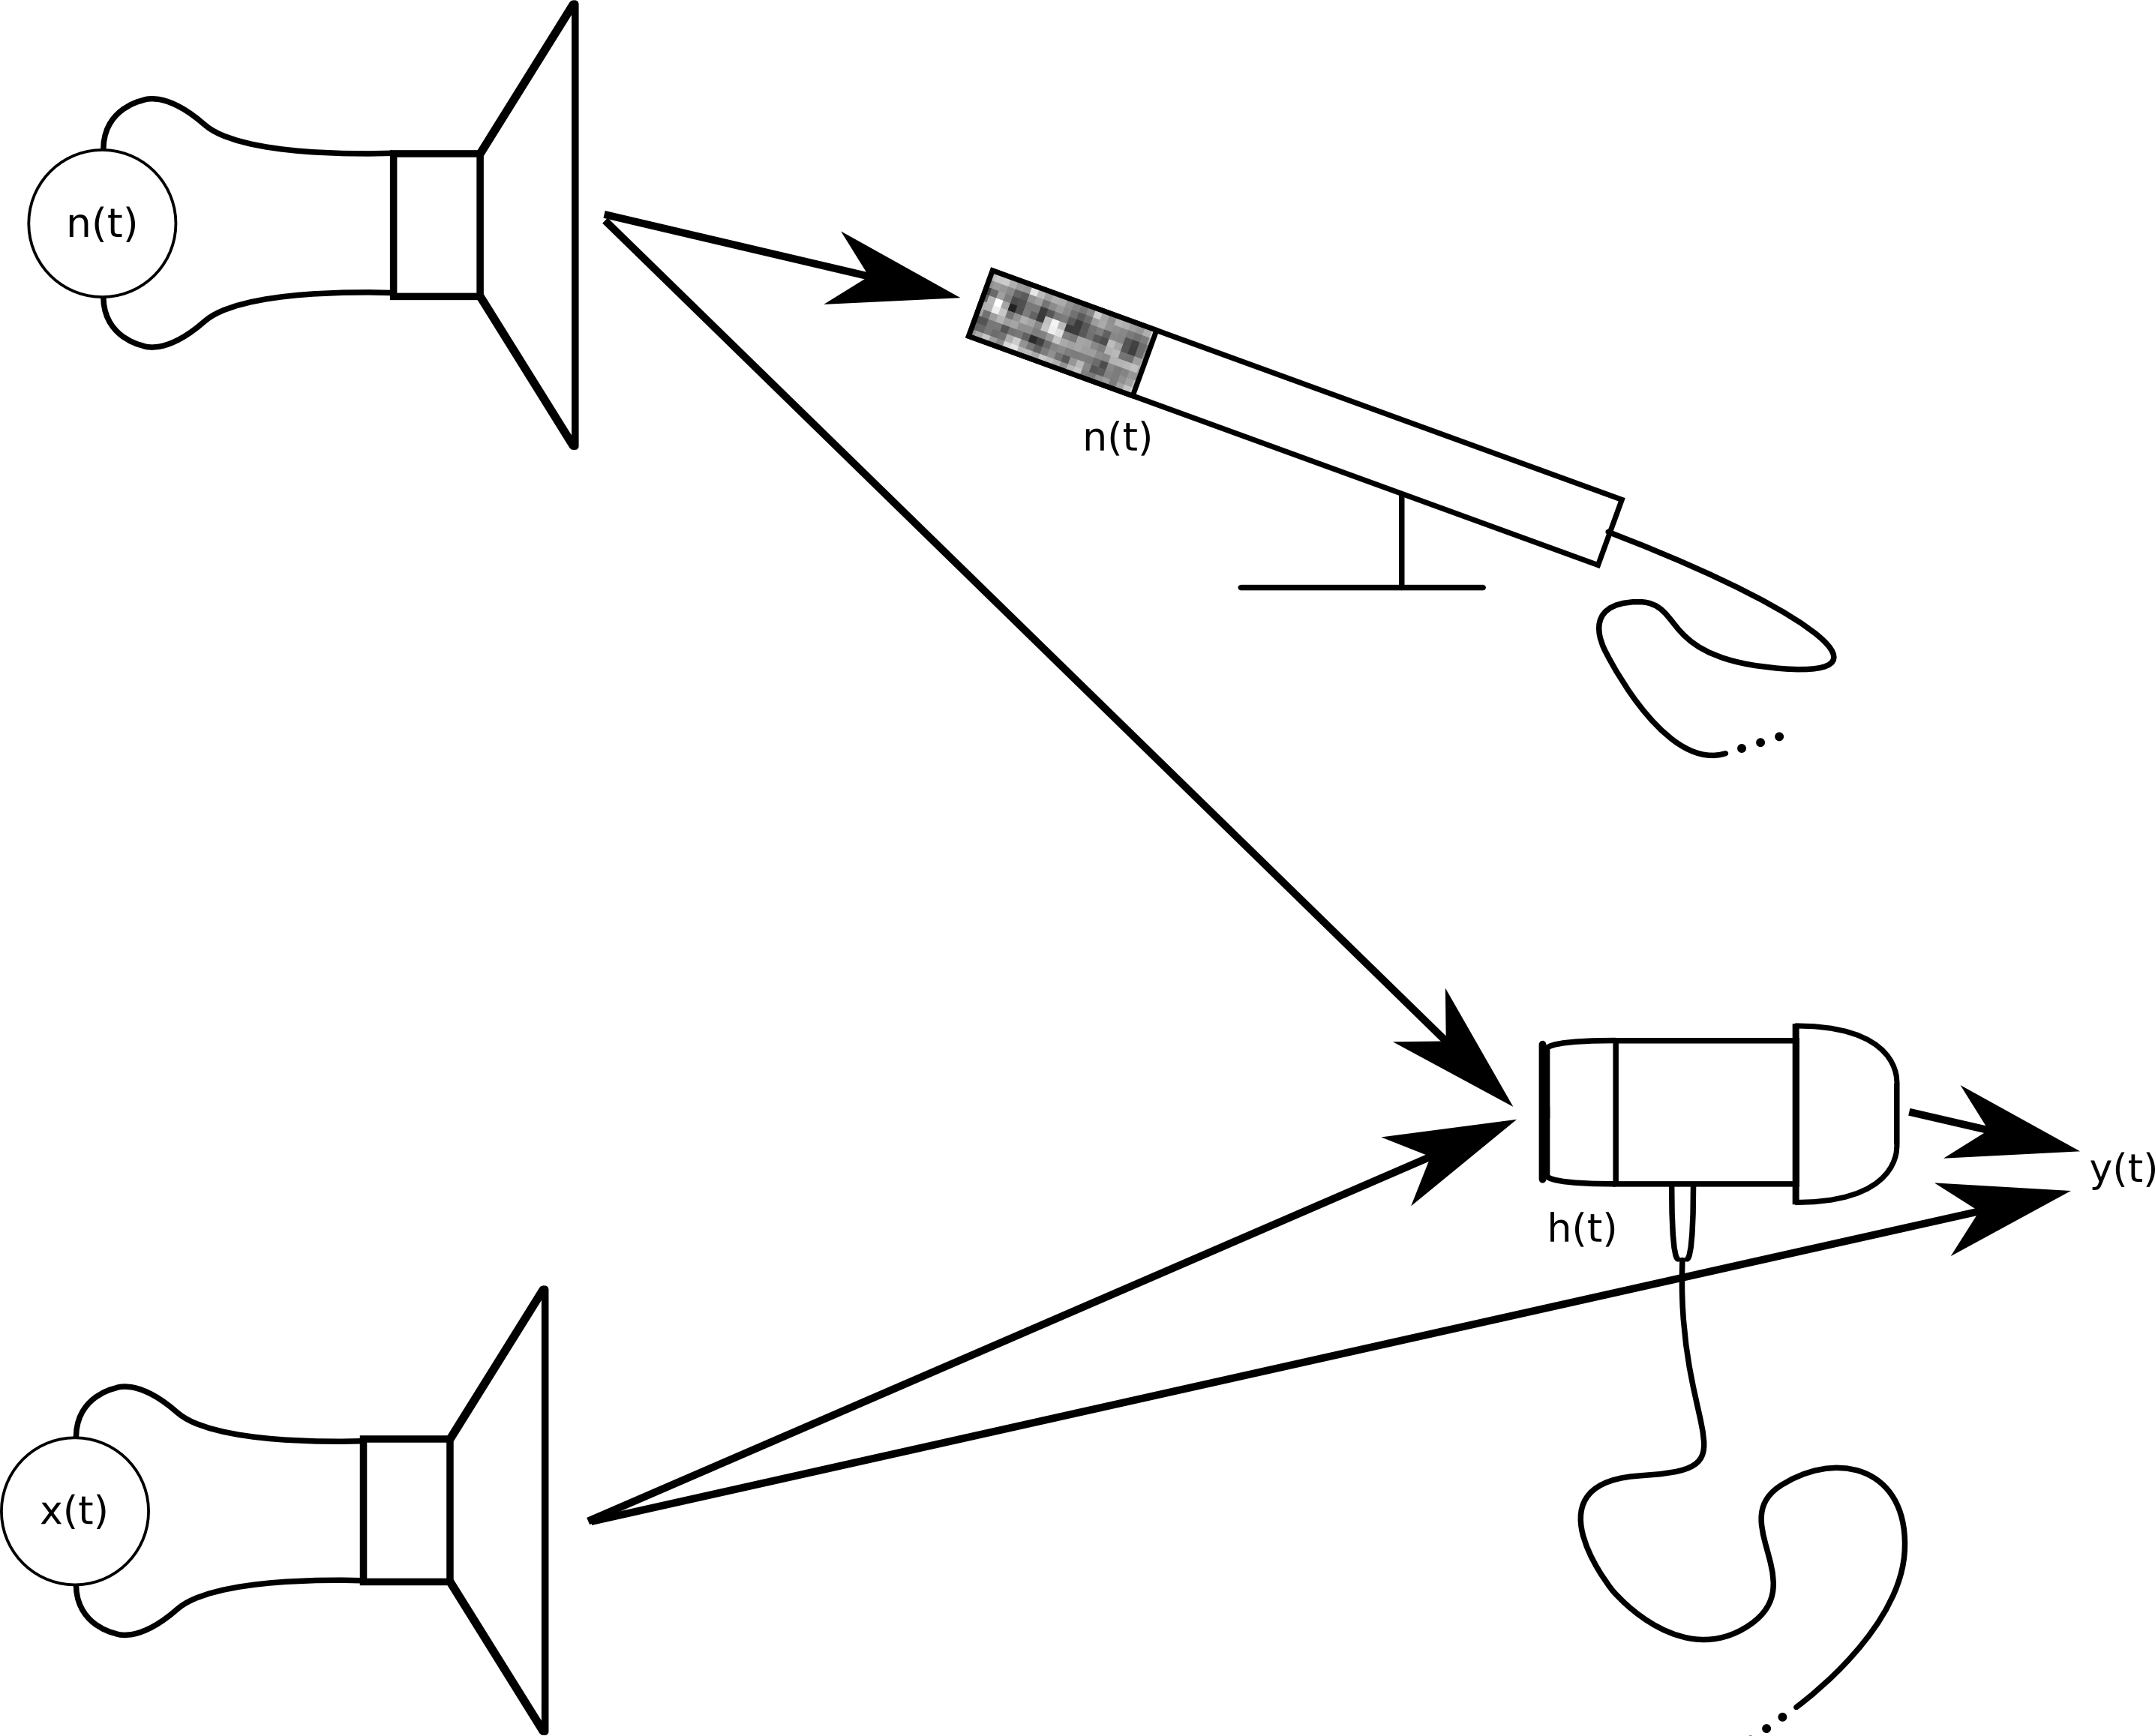
\includegraphics[width=\textwidth]{./img/projdescript.png}
	\caption{An example of the problem this project attempts to solve}
	\label{fig:projdescript}
\end{figure}
\\
\\
For example, a person could be sat in a pub talking with some friends, but there is music blaring out of speakers all around.
It is desirable to be able to hear people talking over the music, however current noise cancelling headphones do not account for this.
This project aims to address situations like this by taking in a noise signal as well as the sound being heard, and then determining how much of the `nuisance' signal is contained in the signal reaching the users' ears.
Once this has been determined, along with any delays or phase shifts being accounted for, a cancelling signal can then be played into the users' ears, resulting in only the unwanted sound being removed.
\\
\\
The basic idea of this can be seen in figure \ref{fig:projdescript}.
Here the music from the speakers is represented by $n(t)$, and the speech represented by $x(t)$.
These may be referred to as the `noise' signal (or `nuisance' signal), and the `desired' signal respectively.
There is also $h(t)$, referred to as the `heard' signal.
This is the sound that would normally reach the ear, and the one that is received by the microphones on the outside of the headphones.
$y(t)$, or the `cancelled' signal is the sound that actually reaches the ear and is the sum of the heard signal and the output from the headphones.
Finally there is the `demanded' signal, $d(t)$.
This is an optional input to allow the user to connect an external device, such as an MP3 player, which will be heard by the user regardless of the other sounds.
It is played directly through the headphones, and therefore forms a component of the cancelled signal. 
